\chapter{Intelligence Gathering}

\section{Overview}

This section describes the \textbf{Intelligence Gathering} activities performed during the penetration test.
\\

Intelligence Gathering consists of performing reconnaissance activities against a target in order to collect as much information as possible. The collected data is then used during the \textbf{Vulnerability Analysis} and \textbf{Exploitation} phases to identify potential attack vectors. The greater the amount of information gathered during this phase, the higher the possibility of detecting viable attack paths.

\section{Target Discovery}

Since the target asset is deployed on a private network using \texttt{DHCP}, it is necessary to identify the IP address assigned to the machine within the network.
\\

The first step is to determine the IP address of the attacking machine. This information will be useful to identify the host during the network scanning phase. The \texttt{ifconfig} command is used for this purpose:
\\

\begin{figure}[H]
    \centering
    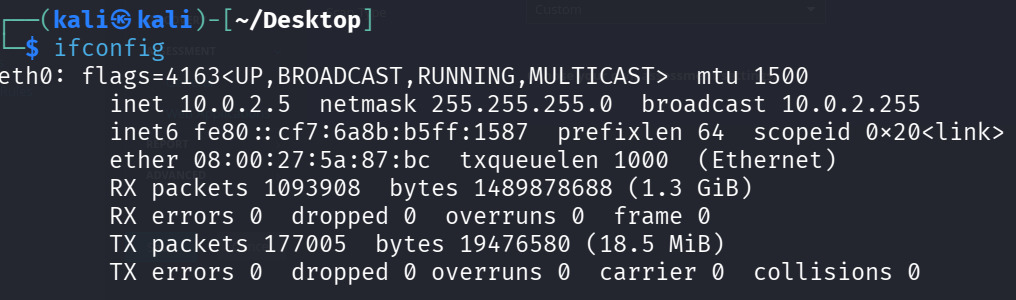
\includegraphics[width=0.75\linewidth]{GlobalAssets/ifconfig.jpeg}
    \caption{\texttt{ifconfig} output}
    \label{ifconfig}
\end{figure}

The IP address of the attacking machine is \texttt{10.0.2.5}.
\\

The next step is to perform a network scan to identify the hosts available within the private network. To accomplish this, \texttt{nmap} is executed with the \texttt{-sn} option:
\\

\begin{figure}[H]
    \centering
    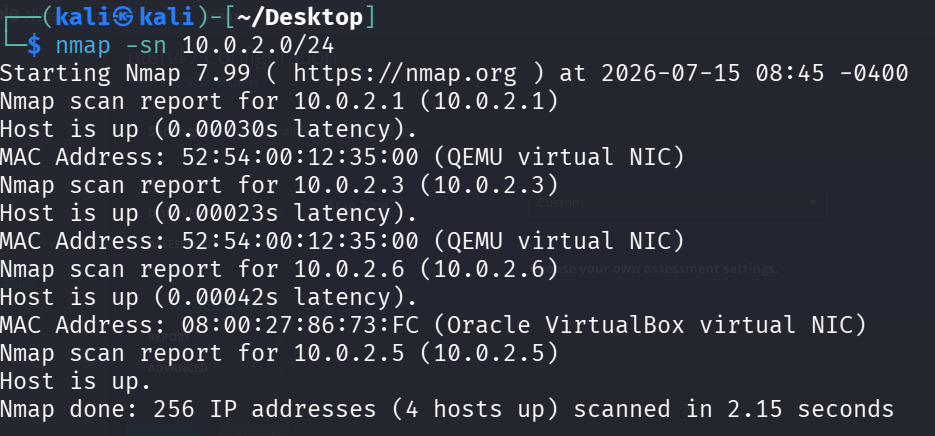
\includegraphics[width=0.75\linewidth]{GlobalAssets/nmap network scan.jpeg}
    \caption{\texttt{nmap} network scan}
    \label{nmapnetworkscan}
\end{figure}

The scan discovered the following hosts:

\begin{description}
    \item[\textbf{\texttt{10.0.2.1}}] This host corresponds to the \textit{VirtualBox NAT Gateway}.
    \item[\textbf{\texttt{10.0.2.3}}] This host corresponds to the \textit{VirtualBox DHCP Server}.
    \item[\textbf{\texttt{10.0.2.5}}] This host corresponds to the attacking machine.
    \item[\textbf{\texttt{10.0.2.6}}] This host corresponds to the target machine.
\end{description}


\section{Enumeration}

A comprehensive scan can now be performed against the target machine in order to collect additional information. To achieve this, \texttt{nmap} is executed with the \texttt{-A} option:
\\

\begin{figure}[H]
    \centering
    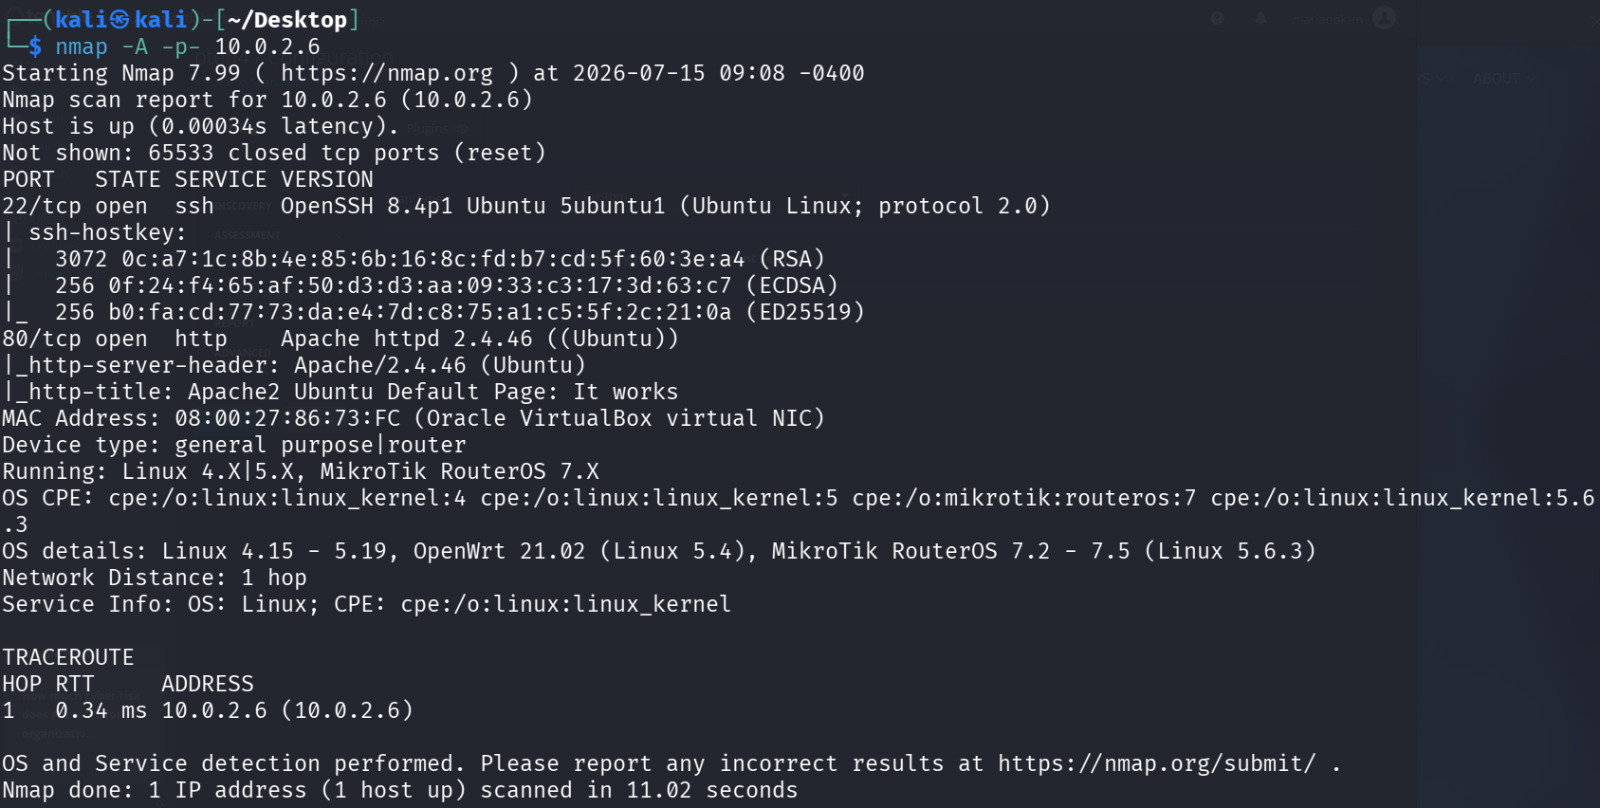
\includegraphics[width=0.75 \linewidth]{GlobalAssets/nmap all scan all ports.jpeg}
    \caption{\texttt{nmap} full scan}
    \label{nmapallscan}
\end{figure}

The scan revealed the following key information:

\begin{itemize}
    \item Port \texttt{22} is open and exposes an \texttt{SSH} service running \texttt{OpenSSH 8.4p1};
    \item Port \texttt{80} is open and exposes an \texttt{Apache2 2.4.46} web server;
    \item The target system is running a \textit{Linux Ubuntu} operating system with a kernel version between \texttt{4.15} and \texttt{5.19}.
\end{itemize}

Since the target exposes a web service, further enumeration activities can be performed against the Apache2 web server to identify possible attack surfaces.
\\

\subsection{Web App Enumeration}

Since the target exposes a web application, additional attack vectors may be discovered through web application enumeration.
\\

The first step is to verify whether the web application can be accessed through a browser:

\begin{figure}[H]
    \centering
    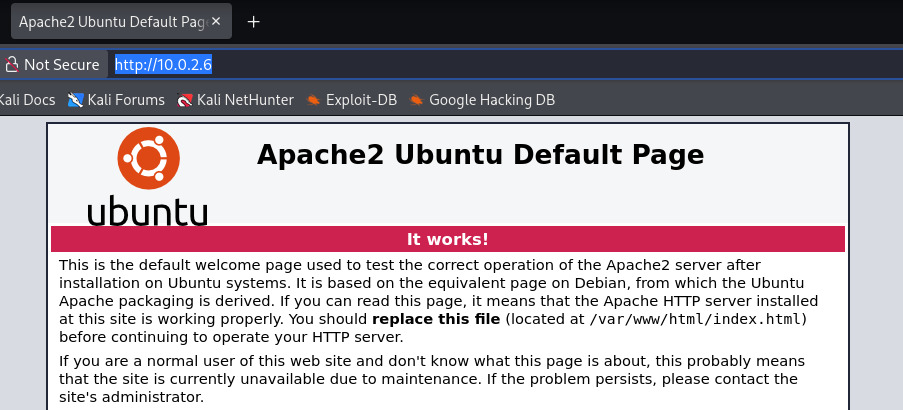
\includegraphics[width=0.75\linewidth]{GlobalAssets/apache default page.jpeg}
    \caption{Apache Default Page}
    \label{apachedefault}
\end{figure}

Accessing \texttt{http://10.0.2.6:80} displays the default \texttt{Apache2 Ubuntu Default Page}.
\\

The next step is to perform web crawling activities in order to identify hidden pages, directories, or files that may expose additional information.
\\

To accomplish this task, \texttt{DirBuster} is used with the wordlist \\ \texttt{/usr/share/dirbuster/wordlists/directory-list-2.3-medium.txt}. Since the assessment is performed within a controlled virtual laboratory environment, a high number of requests can be generated without affecting external systems. Therefore, \texttt{100} threads are configured to maximize the requests-per-second rate:

\begin{figure}[H]
    \centering
    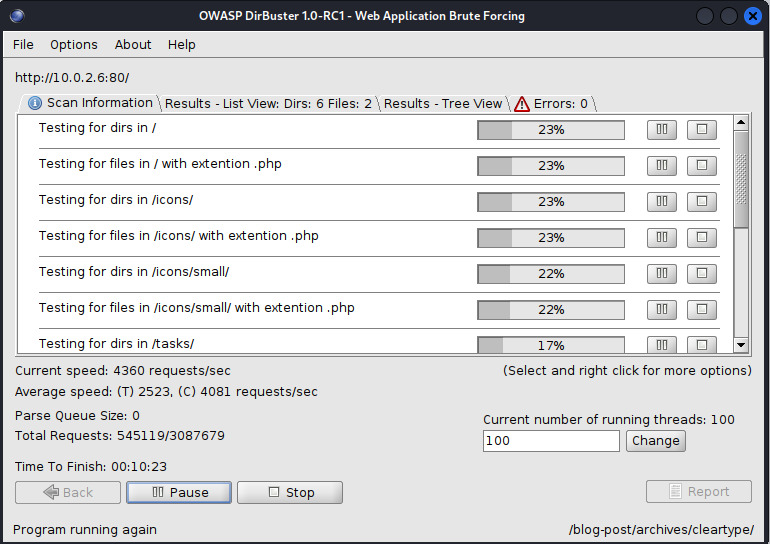
\includegraphics[width=0.75\linewidth]{GlobalAssets/dirbuster executing.jpeg}
    \caption{Execution of \texttt{DirBuster}}
    \label{dirbusterexecution}
\end{figure}

After completing the scan, \texttt{DirBuster} identified several accessible files and directories:
\\

\begin{figure}[H]
    \centering
    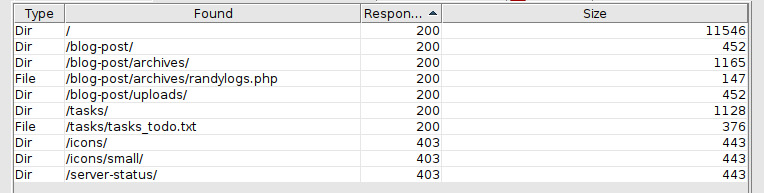
\includegraphics[width=0.75\linewidth]{GlobalAssets/dirbuster result.jpeg}
    \caption{\texttt{DirBuster} results}
    \label{dirbusterresult}
\end{figure}

A total of \textbf{8 directories} and \textbf{2 files} were discovered. Among the identified directories, three returned a \texttt{403 Forbidden} HTTP response code. All remaining resources returned a \texttt{200 OK} response code:

\begin{itemize}
    \item Directory \texttt{/} --- response code \texttt{200};
    \item Directory \texttt{/blog-post/} --- response code \texttt{200};
    \item Directory \texttt{/blog-post/archives/} --- response code \texttt{200};
    \item Directory \texttt{/blog-post/uploads/} --- response code \texttt{200};
    \item Directory \texttt{/tasks/} --- response code \texttt{200};
    \item Directory \texttt{/icons/} --- response code \texttt{403};
    \item Directory \texttt{/icons/small/} --- response code \texttt{403};
    \item Directory \texttt{/server-status/} --- response code \texttt{403};
    \item File \texttt{randylogs.php} --- located in \texttt{/blog-post/archives/} with response code \texttt{200};
    \item File \texttt{tasks\_todo.txt} --- located in \texttt{/tasks/} with response code \texttt{200}.
\end{itemize}

Another directory enumeration scan was performed using \texttt{Gobuster} with the previously mentioned wordlist. The scan identified only the following directories: \texttt{/tasks/}, \texttt{/blog-post/}, and \texttt{/server-status/}.

\begin{figure}[H]
    \centering
    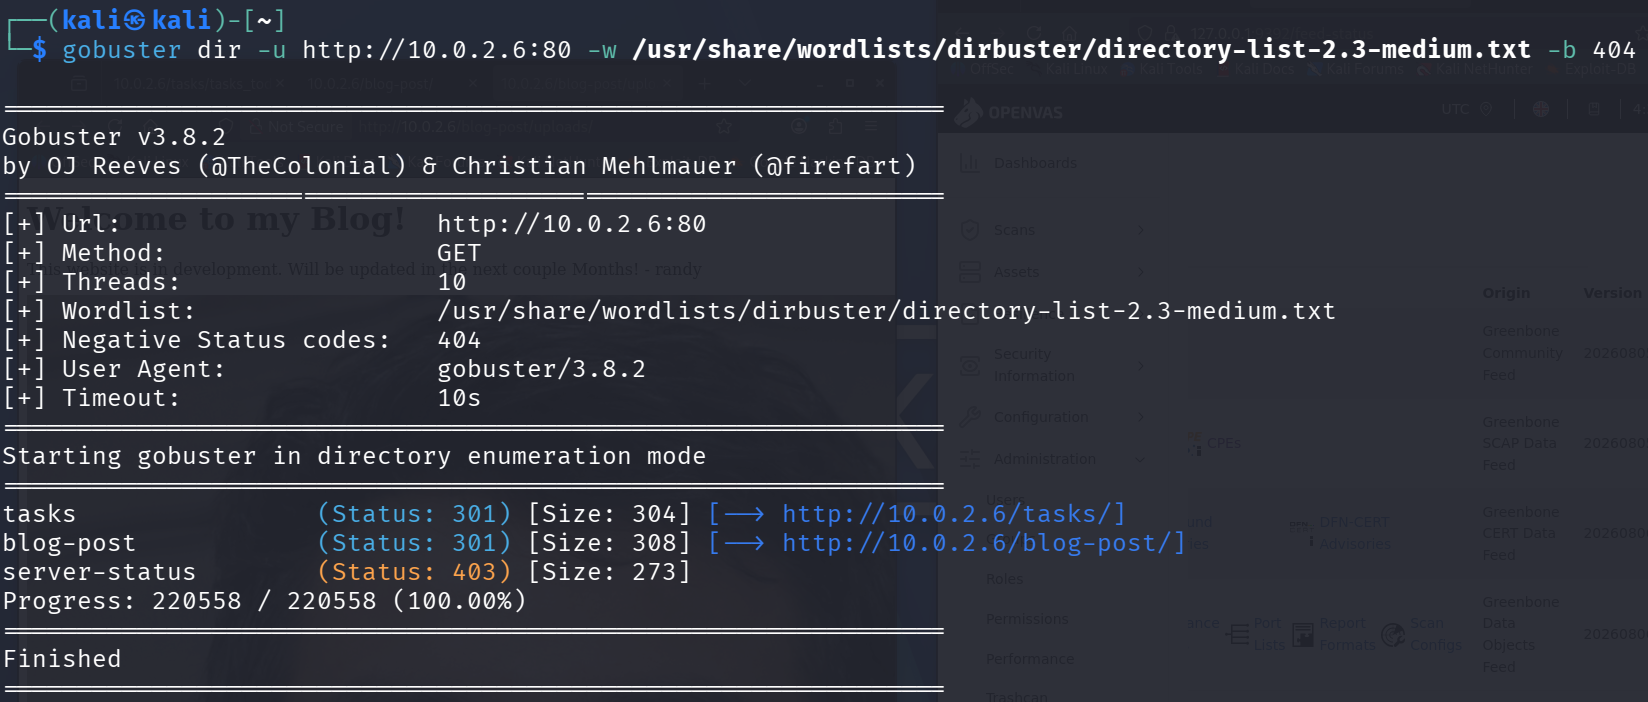
\includegraphics[width=0.75\linewidth]{GlobalAssets/gobuster.png}
    \caption{\texttt{Gobuster} results}
    \label{gobusterresulsts}
\end{figure}

Some of the discovered directories may contain sensitive information that could be useful during the assessment.




